
\begin{opin}{\guscolor}{Gustavo}


\subsubsection{¿Qué es innovar en educación para ti?}
Innovar en educación para mí sería buscar cómo cambiar la forma tradicional de impartir las asignaturas para intentar que los alumnos se sientan más atraídos y puedan retener lo aprendido si no es para el resto de su vidas, al menos durante el mayor tiempo posible y así evitar lo que ocurre en muchos casos de que los alumnos aprueban los exámenes y se olvidan.


\subsubsection{Expectativas iniciales de la asignatura}
Personalmente considero que me encuentro entre ese perfil de alumno que aprueba un examen y se olvida casi por completo de  lo estudiado. Es cierto que esta situación se acentuaba cuando las asignaturas de las que me examinaban eran de memorizar. Con las matemáticas era algo diferente porque era necesario conocer la base para seguir avanzando en los cursos posteriores, los cuales además servían de recordatorio de lo estudiado.


Dicho esto, cuando leí el título de esta asignatura (\textit{Innovación Educativa y TICs aplicadas a la enseñanza de las Matemáticas}) me dio la sensación de que iba a conocer cuáles son las nuevas metodologías de trabajo innovadoras que se están poniendo de moda y que son tan eficaces para el aprendizaje como las metodologías tradicionales. Estas nuevas metodologías docentes incluirían cambios drásticos con respecto a la metodología tradicional. También me imaginaba que se haría mucho hincapié en el uso de las nuevas tecnologías dado que facilita la labor para el docente y es una herramienta muy práctica en el aprendizaje.


Sobre el uso de las TICs en general me gustaría añadir una opinión personal. Tengo la sensación de que hay una tendencia generalizada de pensamiento que opina que con las TICs se va a poder hacer todo. Considero que hay que tener mucho cuidado con el uso de las tecnologías para todo. Las TICs sólo sirven cuando ayudan a realizar una determinada labor. Por poner un ejemplo simple, hay ocasiones en las que las TICs son tan complicadas de usar que no solo no ayudan sino que perjudican.

\end{opin}

\begin{opin}{\victorcolor}{Víctor}

\subsubsection{¿Qué es innovar en educación?}

Hacer las cosas de otra manera. "Si siempre haces lo mismo, no esperes resultados distintos." decía Einstein y para mi innovar es hacer de manera distinta teniendo como objetivo resultados distintos.


Tras comentar en clase la idea de innovación, he descubierto que hay otro aspecto muy importante: que sea un cambio duradero con mucha adopción.
%
Si es un cambio que no mejora las cosas, no es una innovación. 
%
Si nadie está dispuesto a adoptar la nueva forma, tampoco es una innovación.

En esta clase escuché por primera vez el término \index{Educación bulímica}\textbf{educación bulímica}, que significa \textit{Estudio para vomitar en el examen}.


\subsubsection{Expectativas de la asignatura}


Mis expectativas para la asignatura son muy altas, ya que la innovación es fundamental de cara a la profesión docente.
%
Para desarrollarme como buen docente necesito principalmente 2 cosas:
\begin{itemize}
	\item Ser capaz de innovar.
 	\item Estar atento de las innovaciones de otras personas.
 \end{itemize} 

Espero que esta asignatura me ayude a pontenciar mi capacidad innovadora y a conocer recursos con los que innovar en clase, aprovechando las buenas ideas de otras personas.


Estudiando un informe sobre la visión que se tiene de las matemáticas veo resultados que me resultan sorprendentes. 
%
Quien rechaza las mates se hace, no nace. En primaria nadie rechaza las mates, en Secundaria sí.
%
Además, todas las personas reconocen que las matemáticas son realmente útiles, quienes se les dan bien cómo quienes no se les dan bien.
%
A quien le gustan las mates, las consideran fáciles. A quién no le gustan, las consideran difíciles. 50\% de alumnos que rechazan las mates es por culpa de los malos profesores. 30\% de alumnos que no rechazan las mates es gracias a sus profesores. 

Estos datos (y los demás que estuvimos comentando en clase) me hacen darme cuenta de lo fundamental de mi labor y me han hecho tomar conciencia de la responsabilidad que lleva esta profesión. Al fin y al cabo, como dice Ben Parker \textit{un gran poder conlleva una gran responsabilidad}.


\end{opin}

\begin{opin}{\pedrocolor}{Pedro}

\subsubsection{Expectativas iniciales de la asignatura}

En la primera semana del Máster ya fui consciente de mis carencias oratorias, dado mi perfil eminentemente técnico. Por lo tanto, esta asignatura se presenta como un “Recurso” que puede potenciar mis habilidades como educador, por su proximidad al campo científico del que procedo.

Dado que actualmente nos movemos en “la era 3.0”, veo necesario el empleo de nuevas técnicas para llegar mejor al alumnado, permitiendo un mejor desarrollo cognitivo que les permita razonar de forma lógica ante su entorno. 

Mi principal objetivo, al finalizar la asignatura, es conseguir adquirir las nociones necesarias para lograr el empleo de nuevas técnicas educativas y aplicarlas en un futuro a mis alumnos, intentando conseguir con ello una mejor compresión de los conceptos matemáticos.

\subsubsection{¿Qué es innovar en educación?}

Cuando hablamos de “Innovación educativa”, estamos introduciendo cambios en los patrones tradicionales de la educación, que conlleva una mejora del mismo. Para llevarlo a cabo, debemos pasar por un proceso de selección, organización y utilización creativa de los recursos humanos y materiales, que den como resultado los objetivos marcados. (Richland, citado por Moreno, 1995).

Tras la lectura de todas las definiciones de Innovación educativa que han dado alumnos de otros años, me gustaría aportar mi propia definición.

“La innovación educativa nace como resultado de un proceso que consiste en la observación y estudio de manera objetiva de las situaciones que se dan en el aula. Teniendo como resultado final la búsqueda de la mejora del proceso de aprendizaje del alumnado, mediante materiales y técnicas nuevas.

Considero que la mejor manera para demostrar que nuestro intento de Innovación Educativa en el aula tiene efectos positivos en el aprendizaje, es lograr captar la atención del alumno.

Con la llegada de la LOGSE, se comienza a pedir a los profesores de secundaria un conocimiento  didáctico sobre la materia que van a impartir. Sus críticas principales radican en el corto período de formación y la consideración de dicho proceso como un mero trámite.

La LOE habla por primera vez sobre la importancia de enseñar competencias y no contenidos, entendiendo por competencias básicas aquellas habilidades que todos los alumnos deben haber alcanzado al finalizar la Educación Secundaria Obligatoria. Como aspecto negativo, esta ley contempla la posibilidad de pasar de curso con materias suspensas, lo que supone potenciar el error de construir conocimientos justo encima de lagunas arrastradas de cursos anteriores.

Con la implantación del Plan Bolonia, se logra dar al Profesorado de Secundaria la necesaria formación teórica (académica y pedagógica) y práctica.  No obstante, es fundamental que el profesor de matemáticas:

\begin{itemize}
%\vspace{-0.2cm}
\item Se encuentre inmerso en un proceso continuo de actualización (científica y didáctica), lográndose mediante la investigación educativa y acercamiento a nuevas TICs. 
%\vspace{-0.2cm}
\item Se encuentre motivado por la asignatura. 
%\vspace{-0.2cm}
\item Conozca los diferentes enfoques que se puede dar a la asignatura, sin limitarse a formalismos. 
%\vspace{-0.2cm}
\item Elija el metodo adecuado de enseñanza para cada etapa o situación de aprendizaje. 

\end{itemize}

Me llama especialmente la atención los resultados arrojados por los estudios de evaluación educativa (PISA o TIMSS), mostrando un deterioro significativo de la enseñanza matemática pese a las reformas educativas que se han llevado a cabo. Y me pregunto: ¿Qué podemos hacer el profesorado para cambiar esta situación? ¿La utilización de recursos educativos en el aula mejoraría el proceso de enseñanza-aprendizaje? ¿Hace falta ser un experto para el uso básico de TICs?


\begin{minipage}[hbtp]{1.0\linewidth}
\centering
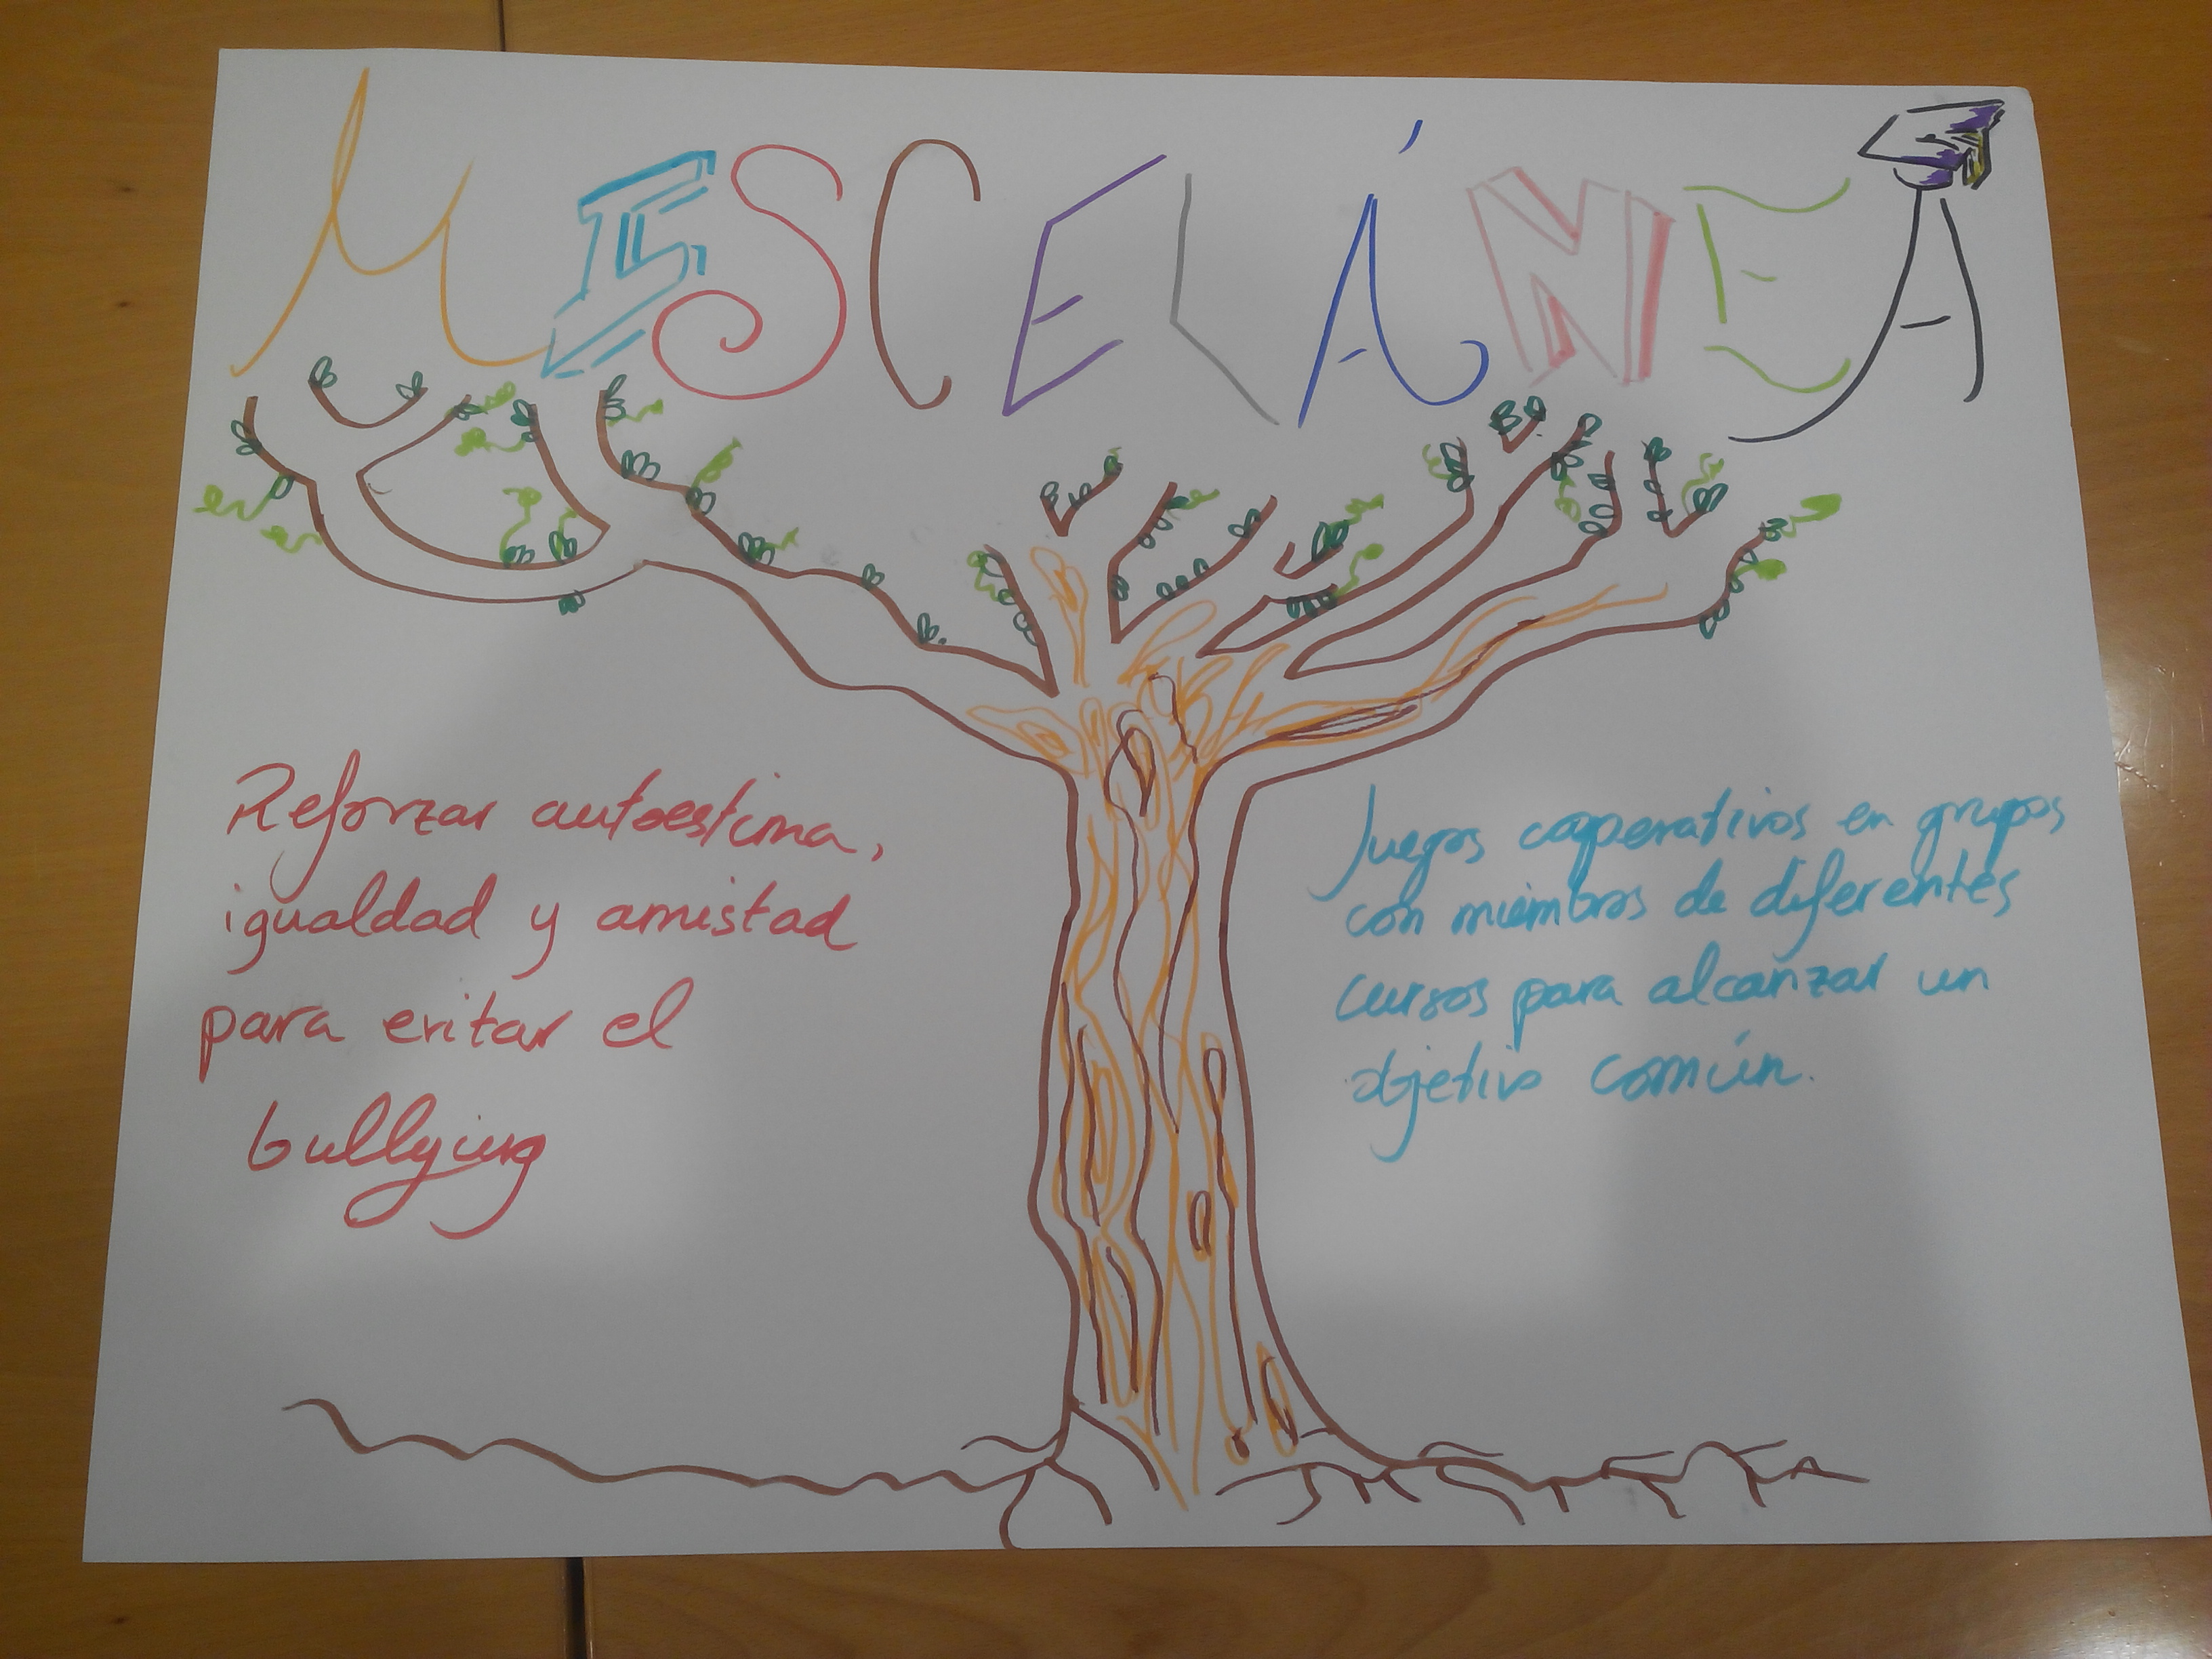
\includegraphics[scale=0.1]{img/pedro1.jpg}
\captionof{figure}{Actividad Jornada Metodologías Activas de educación en el aula con Irene Ros \\ ¿Qué haríais para mejorar la educación?}
\end{minipage}

\end{opin}

\begin{opin}{\virgicolor}{Virginia}

\subsubsection{Expectativas de la asignatura}
Desde el primer momento el nombre de esta asignatura me llamó la atención ya que contiene dos puntos muy importantes en el mundo actual, la innovación y las tecnologías de la información y la comunicación. 

En un mundo en el que la tecnología avanza tan sumamente rápido que compañías tecnológicas importantes están en continuo progreso de tal forma que por ejemplo sacan nuevos dispositivos móviles cada año, no me extraña que esas ganas de innovación y uso de las nuevas tecnologías se aplique a diferentes campos. 

Si bien es cierto es que hasta que leí el nombre de esta asignatura no se me ocurrió pensar en su aplicación a la enseñanza. Desde luego me lleve una grata sorpresa porque creo que puede ser algo muy interesante el transmitir los conocimientos de una forma nueva y diferente usando las tecnologías actuales ya que, en mi época, en los 90, carecíamos de la mayoría de los dispositivos y medios que hay actualmente. 

En definitiva, tengo bastante curiosidad en saber que nos deparará esta asignatura, creo que tiene que ser muy interesante y muy positivo cambiar de alguna forma la enseñanza que hasta ahora conozco con una nueva y mejorada que facilite el aprendizaje. También pienso que debe ser una tarea compleja y que hay mucho por aprender y espero que al finalizar esta asignatura comprenda y sea capaz de aplicar nuevos y diferentes métodos de enseñanza que me permitan mejorar la transmisión de mis conocimientos haciendo que el aprendizaje sea más ameno y divertido y los alumnos estén siempre motivados con una asignatura no muy querida como son las matemáticas.


\subsubsection{Innovar en educación}

En el primer día de clase se entró en contacto por un lado con los conceptos que dan nombre a la asignatura: innovación y tecnologías de la información y la comunicación y por otro lado con el estado actual de la enseñanza tras la evolución de las diferentes leyes de educación.

Antes de escuchar y comprender el significado de la palabra innovación en educación que nos contó Raquel, cada uno definimos cómo entendíamos ese concepto. Mi definición fue la siguiente: innovar en educación es buscar nuevas técnicas o métodos de enseñanza utilizando nuevos recursos como por ejemplo las nuevas tecnologías para conseguir transmitir los conocimientos de una forma nueva y diferente que resulte más atractiva y más fácil de comprender.

Estoy de acuerdo que la innovación tiene que ser objeto de algo planificado, para innovar uno tiene que ser consciente de lo que quiere hacer (introducción de algo nuevo: conceptos, métodos, materiales…) y para qué lo hace (mejorar la enseñanza y el aprendizaje).

Siempre me ha llamado la atención y no positivamente que los gobiernos cambien tan a menudo la ley de educación con lo que eso implica para los estudiantes. A mí me pillo la LOGSE lo que supuso dos cambios de centro en dos años, ya que los institutos tenían que abordar más alumnos, y no estaban preparados cuando me tocó cambiarme, por lo que pase por un centro de “paso”. En mi opinión, cambios de legislación de forma tan frecuente lo único que hacen es despistar más al alumnado y al profesorado, lo que genera huelgas y desmotivación.

Evidentemente creo que España necesita un cambio en el sistema educativo entre otras cosas porque al igual que las personas, la tecnología y la vida evolucionan, la educación también lo tiene que hacer adaptándose a las necesidades actuales.

También me hizo mucho que pensar cuando se trató si era adecuada o no la formación del profesorado. Como es lógico para que los alumnos aprendan de forma adecuada el profesor tiene que tener habilidades psicopedagógicas, pero evidentemente saber de lo que está hablando, es decir, conocer en profundidad la asignatura que imparte. Me resultó impactante que los futuros alumnos de magisterio pudieran suspender matemáticas en selectividad, lo que me hizo reflexionar mucho sobre la formación de los futuros maestros de primaria. En mi opinión, me da la sensación que muchos de los que se apuntan a magisterio se piensan que es una carrera sencilla y de letras en la que no existen las matemáticas, ya que la mayoría de los que hacen magisterio realizan el bachillerato de ciencias sociales o humanidades. Teniendo en cuenta que los primeros seis años de educación escolar en matemáticas están a cargo de los maestros, ¿cómo es posible que no se exijan más conocimientos a los futuros maestros en matemáticas? Conozco maestros de primaria que no saben aplicar un porcentaje en su vida real ni cuando van a las rebajas. Es difícil, que los alumnos entiendan la utilidad de las matemáticas si mucho de los maestros no saben aplicarlas en su vida real. Creo que la labor de un maestro es muy importante y como tal habría que ser más exigentes en su formación.

En vista al problema de matemáticas en primaria, los alumnos llegan a secundaria con un rechazo considerable a la asignatura. Me resultó muy representativa la imagen del círculo vicioso, como dicen en su artículo Hidalgo Alonso, Maroto Sáez y Palacios Pico, de las aptitudes de los estudiantes hacia las matemáticas: dificultad – aburrimiento – suspenso –fatalismo - bajo autoconcepto – desmotivación – rechazo - dificultad. Está claro en matemáticas o en cualquier ámbito de la vida cotidiana que algo que te parece difícil o que te crees que no vales para ello provoca un fuerte rechazo. Así, me parece muy importante en este caso la labor del profesor para conseguir que sus alumnos tengan una actitud positiva a las matemáticas haciéndoles ver que es útil en su vida y que todos ellos tienen capacidad para comprenderla, aptitudes que se tienen que implantar desde primaria y reforzar en secundaria. Por ello, en la primera parte de nuestro trabajo en grupo se quiso hacer hincapié en esto y quisimos tratar el tema de la indefensión aprendida y la motivación para demostrar a los alumnos que si quieren, pueden.

En cuanto a información añadida que Raquel nos incluye en el campus por temas, en este quiero destacar el vídeo de los gansos y el artículo “9 gestos cotidianos que los matemáticos hacemos de otra manera”. Con el vídeo de los gansos lo que se muestra es la importancia de trabajar en grupo, ayudándose los unos a los otros y aprendiendo juntos para lograr un objetivo común. El artículo me resultó muy curioso, destacar lo de no echar la lotería, que me he dado cuenta que es lo mismo que hago yo, que sólo echo la de Navidad por no quedarme con cara de boba si le toca a los demás compañeros del trabajo y a mí no por no comprar el décimo. Me hizo gracia lo de jugar con los números de las matrículas porque me recordó a otra cosa que veo yo en las matrículas, pero es que soy química y no matemática pura por ello lo que yo veo son abreviaciones de productos químicos, por ejemplo cuando veo DNT enseguida me acuerdo del explosivo dinitrotolueno, un símil a lo que hacen los matemáticos con los números.

Otro tema que me hizo reflexionar bastante fue la opción de aplicar nuevos métodos de aprendizaje en la clase que implican la participación activa y colectiva de los alumnos mediante el trabajo por proyectos, sustituyendo la típica clase magistral en la que el profesor suelta todo el temario y luego los alumnos tienen que hacer deberes sin parar y sin apenas entender el qué están haciendo y para qué finalidad. Este nuevo método me abrió la mente a nuevas posibilidades en la educación que yo no imaginaba y que me parecen muy interesantes a la hora de motivar y estimular a los alumnos para que quieran aprender más. Me quedo como conclusión con una frase del educador, psicólogo e investigador Alfredo Hernando autor del blog escuela21: \textit{“La clave, por encima de todo lo demás, es enseñar a los alumnos a pensar por sí mismos. Se trata, según resume Hernando, de plantearles preguntas cuyas respuestas no se puedan googlear"}.

\end{opin}
